%!TEX root = ../thesis.tex
%*******************************************************************************
%*********************************** Eighth Chapter *****************************
%*******************************************************************************

\chapter{Research of the shape changes of the arterial pulses during proximal occlusions}  %Title of the Chapter
\label{chapter apa}

\ifpdf
\graphicspath{{Chapter8/Figs/Raster/}{Chapter8/Figs/PDF/}{Chapter8/Figs/}}
\else
\graphicspath{{Chapter8/Figs/Vector/}{Chapter8/Figs/}}
\fi

The arterial pulses amplitude (APA) are the dynamic component of the impedance plethysmography signal. It lies within the basal impedance which represents about \SI{0.1}{\percent} of the total waveform \cite{anderson1984impedance}. Acquiring these signals can be quite challenging as noise levels could be higher than the actual signal making tough to isolate this waveform. However, obtaining this data provides valuable information about haemodynamics per heartbeat. It has been demonstrated that the shape of the waveform is an indicator of haemodynamic problems in the peripheral circulation. In this chapter, the analysis of the signals aims to differentiate morphological changes between baseline signals and the ones during venous, partial arterial and total occlusion.

As it has been described in the previous chapter, there is a shift in the impedance baseline during each occlusion. However, it is desirable to study the effect that the different kind occlusions of the upper arm produce in the plethysmography waveforms.  This information may provide clues whether an occlusion may be occurring in either the venous or arterial circulation.  The designed iPG device supplies an output port denominated $Z_{AC}$ which provides a high-resolution view of the arterial pulses waveform.  In fact, as shown in the design section \ref{section material envelope}, the signal was filtered and amplified nearly 2500 times to achieve this level of detail. Hence, the waveform obtained provides more in-depth detail and also improves the noise rejection of the signal.

The device produced an excellent result regarding filtering and isolation of the APA waveform. However, undoubtedly some of the noise was also amplified by the hardware. Therefore, further post-processing was required to clean up the plethysmography signal completely. Tighter filters (see table \ref{table:filters}) were applied to remove high and low frequency components. Also, the lower envelope component was also removed and levelled to zero.

The APA waveform produced by the device is inverted as represented by various other plethysmography method such as photoplethysmography. During the systolic cycle, the blood vessels expand allowing more blood volume. Hence, the impedance drops proportionally to the amount of blood because the forearm's segment is more electrically conductive. On the other hand, during the diastolic cycle, blood vessels empty causing a reduction the quantity of blood contained in the segment. As a result, the impedance increases.

The analysis of the plethysmographic wave was performed by averaging the waveforms detected using specialized algorithms able to identify an APA signal. The following section discusses the change of wave shape from a non-occlusion state to an occluded one. At the end of the section, the results of all participants are summarised.

%%********************************** % Section 8.1 ******************************************
\section{Dataset for the arterial amplitude analysis}
\label{section apa 1}
The isolated APA waveforms reproduce the change of volume per heart beat within the sensing electrodes of the iPG device placed in the forearm. The filling of the vessels with blood produces small changes in resistivity that vary with the circulatory cycle (see section \ref{section procedure flow beat}), describing different peaks during a heart cycle.

\begin{figure}[!htpb]
	\centering
	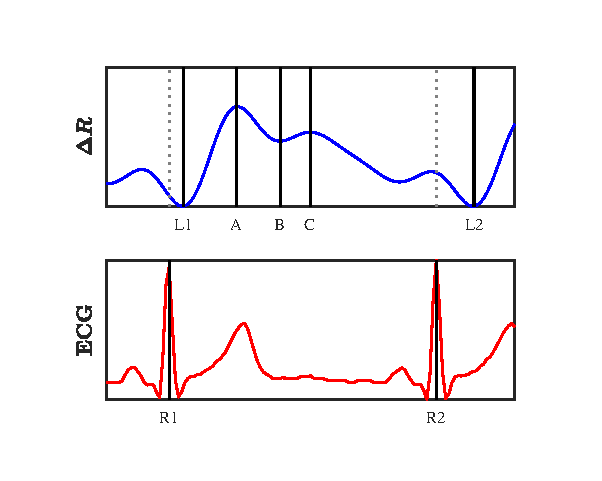
\includegraphics[width=10cm,keepaspectratio]{figure_apa_1}
	\caption[Marker ppoints in an iPG waveform]{Peaks and valleys of an iPG waveform ($\Delta R$) compared to ECG waveform.}
	\label{fig:markers iPG}
\end{figure}

Commonly, an APA wave consists of several identifiable peaks and valleys. Figure \ref{fig:markers iPG} shows a typical impedance plethysmography pulse synchronous with a heartbeat along with a limb. The table \ref{tbl:APA markers} summarises the noticeable markers of the pulse waveforms when compared with an ECG.

\begin{table}[!htpb]
	\caption{Markers on the APA waveform}
	\label{tbl:APA markers}
	\centering
	\begin{tabular}{c p{10cm}}
		\textbf{Marker} & \textbf{Description} \\
		\toprule
		R1 & Peak of the ECG QRS complex before an APA pulse. \\
		L1 & Start of the systolic upslope of the APA signal. Point where  rapid change of impedance occurs. \\
		A & Systolic point. Maximum peak of the APA signal.  \\
		B & Dicrotic notch on the APA wave. \\
		C & Maximum pulse after the dicrotic notch, named diastolic pulse  \\
		R2 & Peak of the ECG QRS complex after the APA pulse.  \\
		L2 & Starting point of the next APA wave. \\
		\bottomrule
	\end{tabular}
\end{table}

An APA wave has to be identified as a valid one to be included in the computational analysis. Therefore, the programmed algorithm starts through the identification of the beginning and the end of a pulse by locating the upslope point $L1$ and $L2$ in the waveform. Once this spot has been identified, the systolic peak $A$ can be placed. Follow, the point $B$ is expected to be a valley with an amplitude below the previous peak. Then, the algorithm looks the following change of slope which is the diastolic peak $C$. In case that any of these conditions were not met, then the algorithm searches the APA wave from the next lower data point, looking for a matching wave pattern again. If a pattern is found ($L1 > A < B > slope change (C) > L2$), then this is count as a fixed wave. If there not match the pulse is marked as missing. Also, to minimise waves with abnormal amplitudes caused by noise, the algorithm calculates the mean peak at $A$ of the last 20 valid APA waves. If the value is greater than \SI{25}{\percent} ($A > A*1.25$) then the wave is discarded.

The table \ref{tbl:detect APA} compiles the amount of APA waves recognised by the algorithm. The column \textit{detected waves} describes the pulses that comply with the profile of an iPG plethysmography wave. The third column shows the pulses that did not match the expected guide; then the algorithm tried to fix them by identifying the pattern in the next slope. As a result, the fixed column shows the total of pulse identified and the last column the ones discarded.

In general, the quality of the APA pulses validated by the iPG device and verified by the algorithm were in average \SI{57.86(1637)}{\percent}. Participants 3, 4 and 8 displayed the highest number of pulses with errors (above \SI{50}{\percent}). However, by performing the fixing method the amount valid peaks improved to a total of \SI{84.94(764)}{\percent}.

\begin{table}[!htbp]
	\caption{Change of amplitude of the waveform at peak A during the transition from baseline to venous occlusion.}
	\label{tbl:detect APA}
	\centering\small
	\begin{tabular}{lrrr>{\columncolor[gray]{0.8}}l>{\columncolor[gray]{0.9}}l}
		\toprule
		& \multicolumn{1}{c}{\textbf{Total}}
		& \multicolumn{1}{c}{\textbf{Detected}} & \multicolumn{1}{c}{\textbf{Waves}}& \multicolumn{1}{c}{\textbf{Fixed}} & \multicolumn{1}{c}{\textbf{Discarded}} \\
		& \multicolumn{1}{c}{\textbf{valleys}} & \multicolumn{1}{c}{\textbf{waves}} & \multicolumn{1}{c}{\textbf{with errors}}& \multicolumn{1}{c}{\textbf{waves}} & \multicolumn{1}{c}{\textbf{waves}} \\
		\midrule
		Participant 1	&1604	& 840 (\SI{52.37}{\percent})	&764 (\SI{47.63}{\percent})	&491 (\SI{30.61}{\percent})	&273 (\SI{17.02}{\percent})\\
		Participant 2	&1689	&1159 (\SI{68.62}{\percent})	&530 (\SI{31.38}{\percent})	&409 (\SI{24.22}{\percent})	&121 ( \SI{7.16}{\percent})\\
		Participant 3	&1651	& 699 (\SI{42.34}{\percent})	&952 (\SI{57.66}{\percent})	&695 (\SI{42.10}{\percent})	&257 (\SI{15.57}{\percent})\\
		Participant 4	&1625	& 645 (\SI{39.69}{\percent})	&980 (\SI{60.31}{\percent})	&562 (\SI{34.58}{\percent})	&418 (\SI{25.72}{\percent})\\
		Participant 5	&1664	&1199 (\SI{72.06}{\percent})	&465 (\SI{27.94}{\percent})	&345 (\SI{20.73}{\percent})	&120 ( \SI{7.21}{\percent})\\
		Participant 6	&1745	& 936 (\SI{53.64}{\percent})	&809 (\SI{46.36}{\percent})	&471 (\SI{26.99}{\percent})	&338 (\SI{19.37}{\percent})\\
		Participant 7	&1907	&1654 (\SI{86.73}{\percent})	&253 (\SI{13.27}{\percent})	&146 ( \SI{7.66}{\percent})	&107 ( \SI{5.61}{\percent})\\
		Participant 8	&1651	& 784 (\SI{47.49}{\percent})	&867 (\SI{52.51}{\percent})	&491 (\SI{29.74}{\percent})	&376 (\SI{22.77}{\percent})\\
		\bottomrule
	\end{tabular}
\end{table}

From these data, the changes during each occlusion among the points $A$, $B$ and $C$  were examined. The following analysis centres in the changes of impedance amplitude all along the different regions of the experiment, and the change of area of the waveform before and after the dicrotic notch point ($B$).


%%********************************** % Section 8.2 ******************************************
\section{Changes of the plethysmography waveform during different occlusions}
\label{section apa 2}
From the detection of the APA waveforms are possible to analyse the change of the shape form independently. For this, an average waveform was computed for each of the regions during the experiment. The following section details the changes for each of the points of interest. 

%%********************************** % Section 8.2.1 ******************************************
\subsection{Plethysmography waveform change during venous occlusion}
\label{section apa 2.1}
The analysis performed in this section corresponds to the APA waveforms captured during baseline in region 1 (\SIrange{0}{300}{\second}), venous occlusion (\SIrange{300}{480}{\second}) and return to control signal (\SIrange{480}{780}{\second}).  The previous section described the method how the valid pulses were collected. Consequently, all the valid pulses were grouped and aligned per region calculating the average waveform.


%This method allows multifigures being aligned using subcaptionbox
\begin{figure*}[!htbp]
	\centering
	\null\hfill%
	\subcaptionbox{Average APA waveform for baseline region 1 (\SIrange{0}{300}{\second})\label{fig:iPG_venous_baseline}}
	[0.48\textwidth]{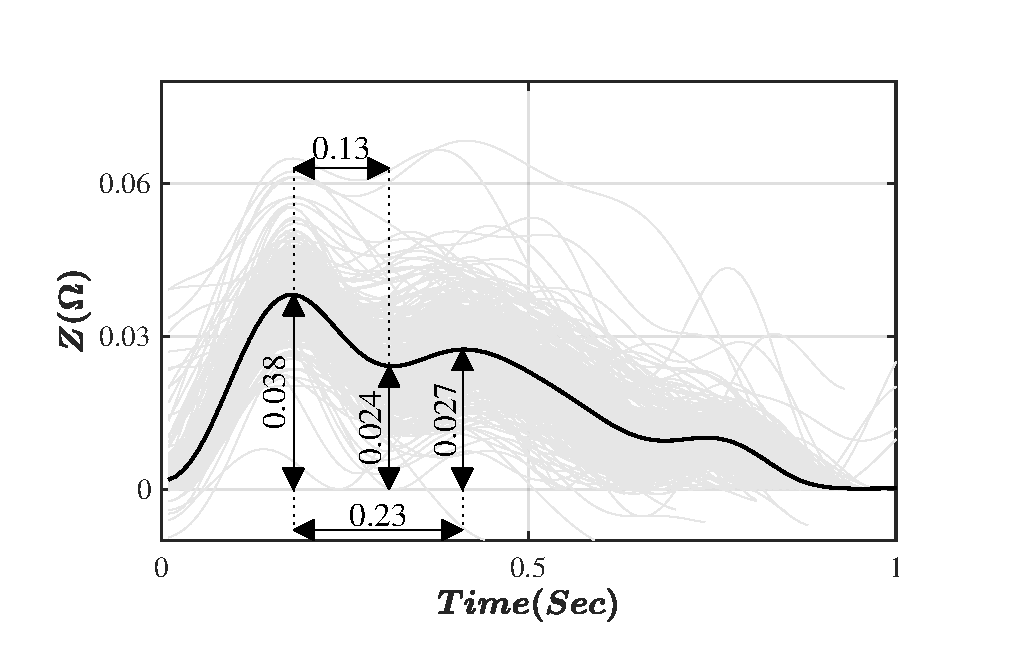
\includegraphics[width=0.48\textwidth, trim={0.5cm 0cm 1.5cm 0 cm}, clip]{figure_apa_2a}}%
	\hfill%
	\subcaptionbox{Average APA waveform during venous occlusion region 2 (\SIrange{300}{480}{\second})\label{fig:iPG_venous_occlusion}}
	[0.48\textwidth]{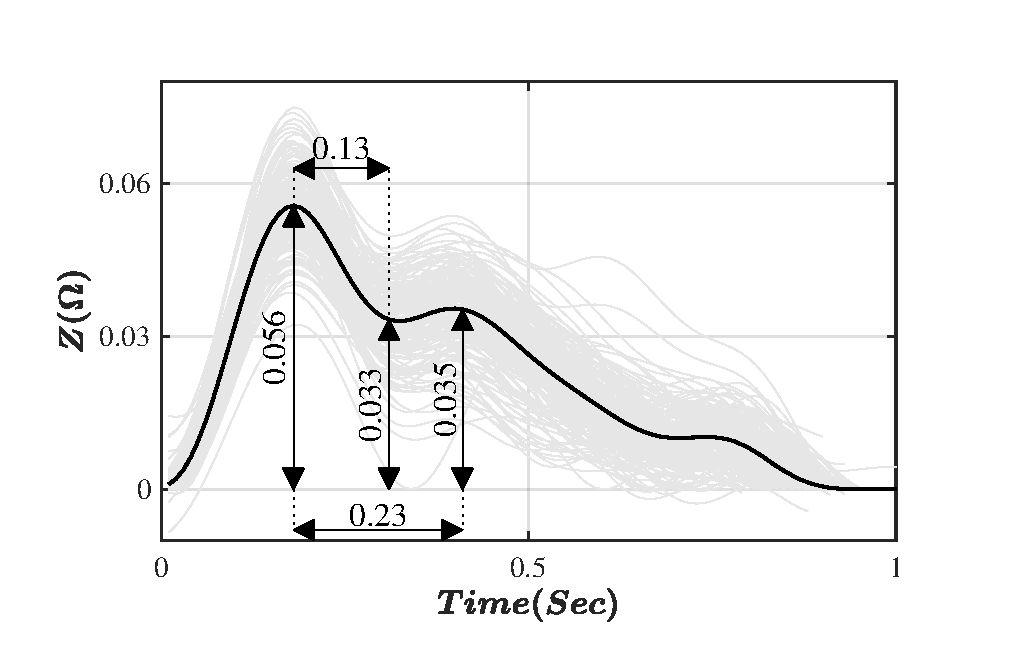
\includegraphics[width=0.48\textwidth, trim={0.5cm 0cm 1.5cm 0 cm}, clip]{figure_apa_2b}}%
	\hfill\null%
	\caption{Plethysmography waveform of the participant seven between baseline and venous occlusion}
	\label{fig:iPG_venous}
	
	\vspace{1cm}
	
	\null\hfill%
	\subcaptionbox{Change of amplitude of the waveform at point A.\label{fig:change A venous}}
	[0.48\textwidth]{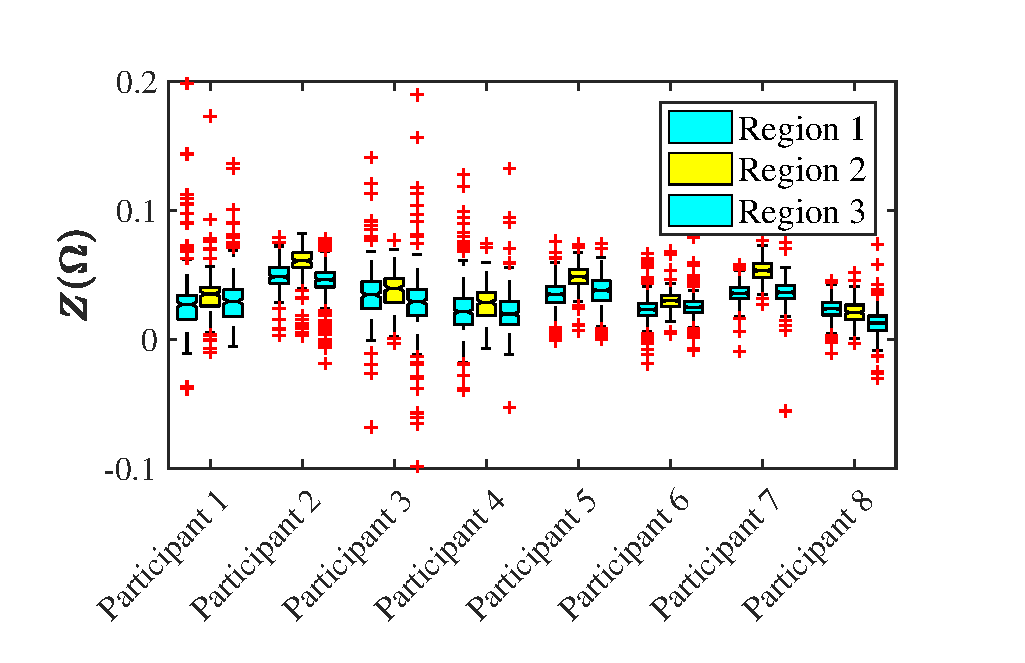
\includegraphics[width=0.45\textwidth, trim={0.5cm 0cm 1.5cm 0 cm}, clip]{figure_apa_3a}}%
	\hfill%
	\subcaptionbox{Change of amplitude of the waveform at point B.\label{fig:change B venous}}
	[0.48\textwidth]{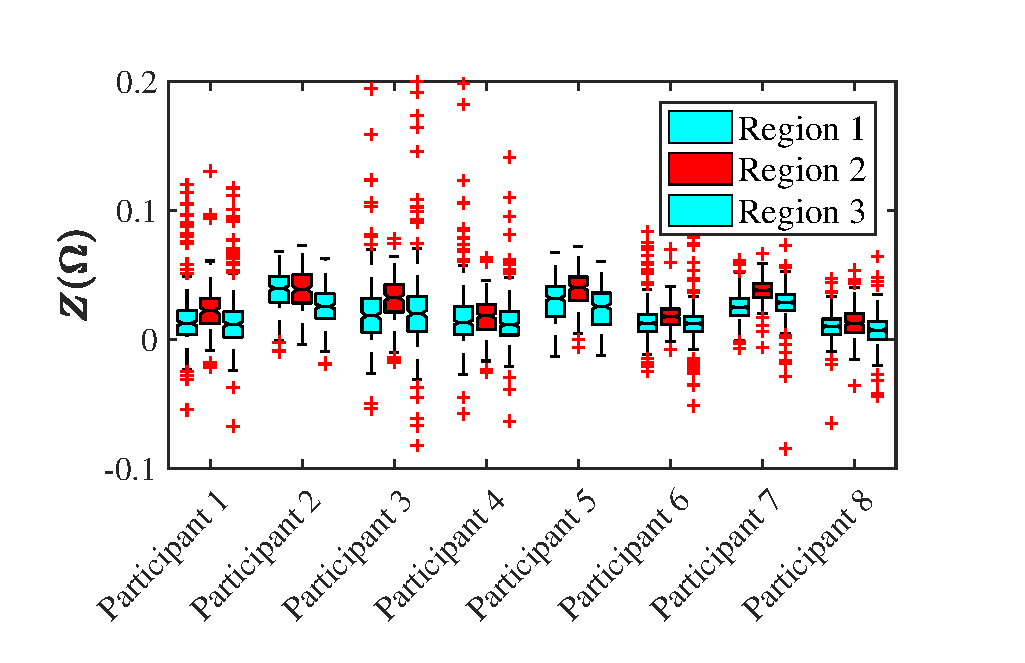
\includegraphics[width=0.45\textwidth, trim={0.5cm 0cm 1.5cm 0 cm}, clip]{figure_apa_3b}}%
	\hfill%
	\subcaptionbox{Change of amplitude of the waveform at point C.\label{fig:change C venous}}
	[0.48\textwidth]{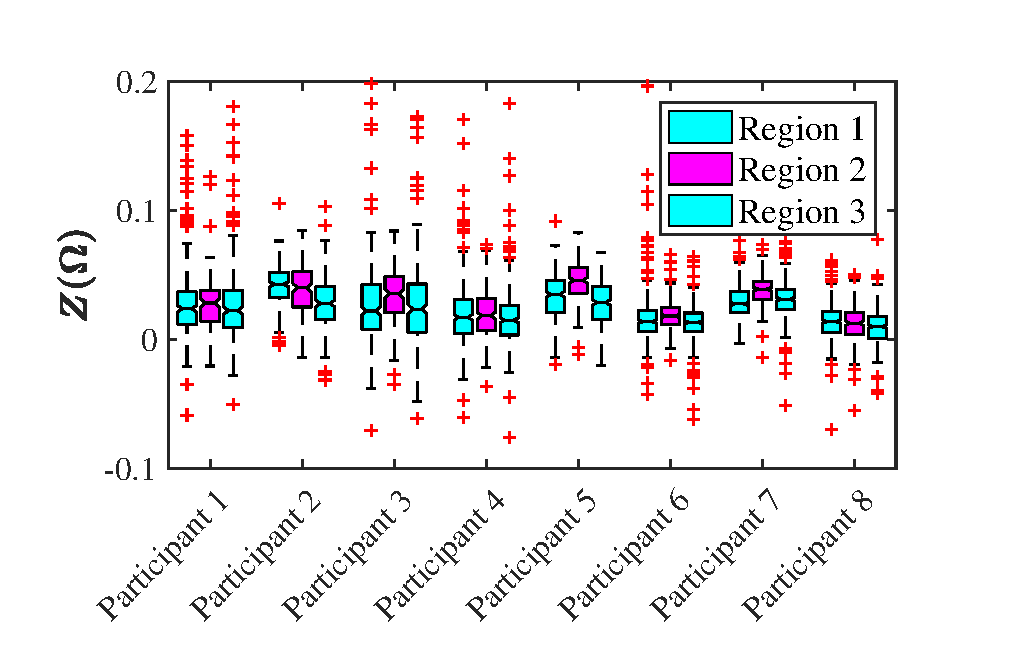
\includegraphics[width=0.45\textwidth, trim={0.5cm 0cm 1.5cm 0 cm}, clip]{figure_apa_3c}}%
	\null%
	\caption{Changes of the impedance peak values during baseline, venous occlusion and return to baseline for points A,B and C.}
	\label{fig:iPG change points venous}
\end{figure*}

Figure \ref{fig:iPG_venous_baseline} shows an impedance plethysmography waveform calculated from one of the participants during baseline and venous occlusion, with indicators of their amplitudes at the different points of interest. Some of the markers show the calculation of the distance between systolic peak (Point A) to dicrotic notch (Point B) and diastolic peak (Point C), as well as, the amplitude for each of these markers. The distance between (A $\rightarrow$ B) and (A $\rightarrow$ C) was later transposed into the occlusion wave to identify their values during the VOP test.

Clearly,  from a qualitative point of view, one can notice that there is a difference in the morphology of the waveform during the occlusion.  Indeed, figure \ref{fig:iPG change points venous} shows the change of the amplitude at these points for every participant and the return to baseline after the cuff pressure was released. A complete analysis of the change at each point is detailed as follows.

\subsubsection{Changes in systolic peak (Point A)}
\label{section apa 2.1.1}
Figure \ref{fig:change A venous} shows the statistical variation of the systolic peak magnitude (point A) during the three conditions of the test baseline-occlusion-baseline. After inflating the cuff below the diastolic pressure, most of the APA signals displayed an increase of the impedance magnitude of this peak. Indeed, as detailed in table \ref{tbl:change A venous}, \SI{87}{\percent} of the participants showed an increment in electrical resistance during venous occlusion of about \SI{31.80}{\percent}, only participant 8 was an exception where his/her impedance decreased in \SI{-12.01}{\percent}. Then, when the cuff's pressure was released, all the participants showed a decline of the peak value with an average of \SI{-32.21}{\percent}, returning to similar baseline values before the venous occlusion.

\begin{table}[!htbp]
	\caption[Change of amplitude of the waveform at peak A during the transition baseline-venous occlusion-baseline.]{Change of amplitude of the waveform at peak A during the transition from baseline (region 1), venous occlusion (region 2) and return to baseline (region 3). The column change shows the percentile variations between the different regions.}
	\label{tbl:change A venous}
	\centering\small
\begin{tabular}{l
				*{3}{S[table-format=1.4]@{\,\( \pm \)\,}S[table-format=1.4]} %Format for Z+-std
		       >{\columncolor[gray]{0.8}}c>{\columncolor[gray]{0.9}}c}
	\toprule
	& \multicolumn{2}{c}{\multirow{2}{*}{\textbf{Baseline [\si{\ohm}]}}}
	& \multicolumn{2}{c}{\multirow{2}{*}{\textbf{Occlusion [\si{\ohm}]}}}
	& \multicolumn{2}{c}{\multirow{2}{*}{\textbf{Baseline [\si{\ohm}]}}}
	& \multicolumn{2}{c}{\textbf{Change}} \\
	& \multicolumn{2}{c}{}
	& \multicolumn{2}{c}{}
	& \multicolumn{2}{c}{}
	&\textbf{R1-R2}&\textbf{R2-R3}\\\midrule
    Participant 1 & 0.0270 & 0.0233 & 0.0353 & 0.0191 & 0.0295 & 0.0305 & 30.49 \% & -21.41 \% \\
	Participant 2 & 0.0485 & 0.0102 & 0.0609 & 0.0140 & 0.0462 & 0.0449 & 25.50 \% & -30.24 \% \\
	Participant 3 & 0.0345 & 0.0351 & 0.0397 & 0.0144 & 0.0292 & 0.0294 & 14.96 \% & -30.55 \% \\
	Participant 4 & 0.0214 & 0.0303 & 0.0289 & 0.0139 & 0.0197 & 0.0222 & 35.17 \% & -43.11 \% \\
	Participant 5 & 0.0352 & 0.0112 & 0.0485 & 0.0098 & 0.0382 & 0.0376 & 37.99 \% & -29.20 \% \\
	Participant 6 & 0.0232 & 0.0105 & 0.0300 & 0.0124 & 0.0249 & 0.0251 & 29.16 \% & -21.77 \% \\
	Participant 7 & 0.0357 & 0.0080 & 0.0534 & 0.0081 & 0.0365 & 0.0365 & 49.33 \% & -47.17 \% \\
	Participant 8 & 0.0238 & 0.0094 & 0.0209 & 0.0091 & 0.0128 & 0.0127 &-12.01 \% & -34.27 \% \\ \bottomrule
\end{tabular}
\end{table}


\subsubsection{Changes in dicrotic notch peak (Point B)}
\label{section apa 2.1.2}
The dicrotic notch (point B) is located between the systolic (point A) and diastolic peaks (point C) as represented in figure \ref{fig:markers iPG}.  Similarly, as the changes experienced by the systolic peak during this part of the experiment, the point B also increased in its magnitude. After that, when the cuff's pressure was released the amplitude at this location returned to an amplitude quite close to the baseline.

According to the data shown on Table \ref{tbl:change B venous}, one can see that most of the participants (\SI{87.5}{\percent}) showed an increase in the magnitude of their dicrotic notch point. Certainly, between those who experienced this increment, the impedance changed roughly \SI{47.73}{\percent} compared to the measurement at region 1. However, partaker two noted a slight decrease in her measured impedance \SI{-2.06}{\percent} which was not very significant compared to the others. In contrast, after releasing the upper arms blockage, all the participants experienced a drop of their point B magnitude of about  \SI{-51.68}{\percent}.

\begin{table}[!htbp]
	\caption{Change of amplitude of the waveform at peak B during the transition from baseline to venous occlusion.}
	\label{tbl:change B venous}
	\centering\small
	\begin{tabular}{l
					*{3}{S[table-format=1.4]@{\,\( \pm \)\,}S[table-format=1.4]} %Format for Z+-std
					>{\columncolor[gray]{0.8}}c>{\columncolor[gray]{0.9}}c}
	\toprule
	& \multicolumn{2}{c}{\multirow{2}{*}{\textbf{Baseline [\si{\ohm}]}}}
	& \multicolumn{2}{c}{\multirow{2}{*}{\textbf{Occlusion [\si{\ohm}]}}}
	& \multicolumn{2}{c}{\multirow{2}{*}{\textbf{Baseline [\si{\ohm}]}}}
	& \multicolumn{2}{c}{\textbf{Change}} \\
	& \multicolumn{2}{c}{}
	& \multicolumn{2}{c}{}
	& \multicolumn{2}{c}{}
	&\textbf{R1-R2}&\textbf{R2-R3}\\\midrule
	Participant 1 & 0.0126 & 0.0231 & 0.0223 & 0.0195 & 0.0119 & 0.0153 & 76.94 \% & -82.52 \% \\
	Participant 2 & 0.0397 & 0.0144 & 0.0388 & 0.0167 & 0.0257 & 0.0252 & -2.06 \% & -33.19 \% \\
	Participant 3 & 0.0184 & 0.0315 & 0.0323 & 0.0181 & 0.0200 & 0.0224 & 75.98 \% & -67.36 \% \\
	Participant 4 & 0.0130 & 0.0294 & 0.0183 & 0.0149 & 0.0113 & 0.0138 & 40.21 \% & -53.52 \% \\
	Participant 5 & 0.0319 & 0.0158 & 0.0402 & 0.0138 & 0.0254 & 0.0237 & 25.92 \% & -46.26 \% \\
	Participant 6 & 0.0127 & 0.0138 & 0.0177 & 0.0161 & 0.0124 & 0.0128 & 39.75 \% & -41.55 \% \\
	Participant 7 & 0.0250 & 0.0108 & 0.0382 & 0.0092 & 0.0287 & 0.0276 & 52.71 \% & -37.97 \% \\
	Participant 8 & 0.0102 & 0.0111 & 0.0125 & 0.0117 & 0.0073 & 0.0071 & 22.58 \% & -51.08 \% \\
 \bottomrule
	\end{tabular}
\end{table}

\subsubsection{Changes in diastolic peak (Point C)}
\label{section apa 2.1.3}
The last peak analysed corresponds to the point C or diastolic peak of the waveform. Again, figure \ref{fig:change C venous} shows that most of the participants (\SI{71.4}{\percent}) showed an increase in the magnitude at this point of about \SI{31.92}{\percent} compared to region 1. Only, participants 2 and 8 described a slight decrease of their impedance in an average of \SI{-7.97}{\percent}. Table \ref{tbl:change C venous} shows the mean values of the impedance at this location in the waveform. In contrast, after releasing the upper arm's pressure, all the participants experienced a decrease in their diastolic peak impedance, with an average of \SI{-32.33}{\percent}. Hence, the diastolic peak returned to values similar to the baseline, except for the ones that experience a decrease in resistance during the occlusion.

\begin{table}[!htbp]
	\caption{Change of amplitude of the waveform at peak C during the transition from baseline to venous occlusion.}
	\label{tbl:change C venous}
	\centering\small
	\begin{tabular}{l
					*{3}{S[table-format=1.4]@{\,\( \pm \)\,}S[table-format=1.4]} %Format for Z+-std
					>{\columncolor[gray]{0.8}}c>{\columncolor[gray]{0.9}}c}
	\toprule
	& \multicolumn{2}{c}{\multirow{2}{*}{\textbf{Baseline [\si{\ohm}]}}}
	& \multicolumn{2}{c}{\multirow{2}{*}{\textbf{Occlusion [\si{\ohm}]}}}
	& \multicolumn{2}{c}{\multirow{2}{*}{\textbf{Baseline [\si{\ohm}]}}}
	& \multicolumn{2}{c}{\textbf{Change}} \\
	& \multicolumn{2}{c}{}
	& \multicolumn{2}{c}{}
	& \multicolumn{2}{c}{}
	&\textbf{R1-R2}&\textbf{R2-R3}\\\midrule
    Participant 1 & 0.0238 & 0.0281 & 0.0283 & 0.0260 & 0.0224 & 0.0286 & 18.81 \% & -24.75 \% \\
	Participant 2 & 0.0429 & 0.0150 & 0.0401 & 0.0191 & 0.0279 & 0.0278 & -6.48 \% & -28.45 \% \\
	Participant 3 & 0.0221 & 0.0397 & 0.0355 & 0.0219 & 0.0236 & 0.0310 & 60.85 \% & -53.94 \% \\
	Participant 4 & 0.0171 & 0.0380 & 0.0184 & 0.0174 & 0.0149 & 0.0178 &  7.42 \% & -20.30 \% \\
	Participant 5 & 0.0350 & 0.0175 & 0.0459 & 0.0151 & 0.0287 & 0.0279 & 31.16 \% & -49.18 \% \\
	Participant 6 & 0.0138 & 0.0212 & 0.0182 & 0.0251 & 0.0133 & 0.0151 & 31.53 \% & -35.22 \% \\
	Participant 7 & 0.0276 & 0.0127 & 0.0391 & 0.0111 & 0.0312 & 0.0309 & 41.77 \% & -28.58 \% \\
	Participant 8 & 0.0138 & 0.0140 & 0.0125 & 0.0163 & 0.0100 & 0.0096 & -9.47 \% & -18.24 \% \\

	\bottomrule
	\end{tabular}
\end{table}

%%********************************** % Section 8.2.2 ******************************************
\subsection{Plethysmography waveform change during partial arterial occlusion}
\label{section apa 2.2}
During the partial occlusion of the brachial artery, similarly to venous occlusion, most of the participants also showed a change in the shape of their waveforms. The analysis of this section resembles the baseline time in region 3 (\SIrange{480}{780}{\second}), three minutes of partial venous occlusion in region 4 (\SIrange{780}{960}{\second}) and return to baseline region 5 (\SIrange{960}{1260}{\second}). The cuff was inflated to the pressure presented in column \textit{Occlusion 2} in Table \ref{tbl: venous occlusions}, laying between diastolic ans systolic pressures.

Figure \ref{fig:iPG arterial} shows the average waveform of all the signals aligned at baseline and during the arm's occlusion for one of the participants. As is evident from the plot, there is an increase in the systolic peak (point A) and a reduction in the diastolic peak at point C). Figure \ref{fig:iPG change points arterial} also features the impedance change in each participant during the three regions of the experiment. The following sections will describe in detail the changes to each of the spots.

%This method allows multifigures being aligned using subcaptionbox
\begin{figure*}
	\centering
	\null\hfill%
	\subcaptionbox{Average plethysmography waveform during venous occlusion region 3 (\SIrange{480}{780}{\second})\label{fig:iPG arterial baseline}}
	[0.45\textwidth]{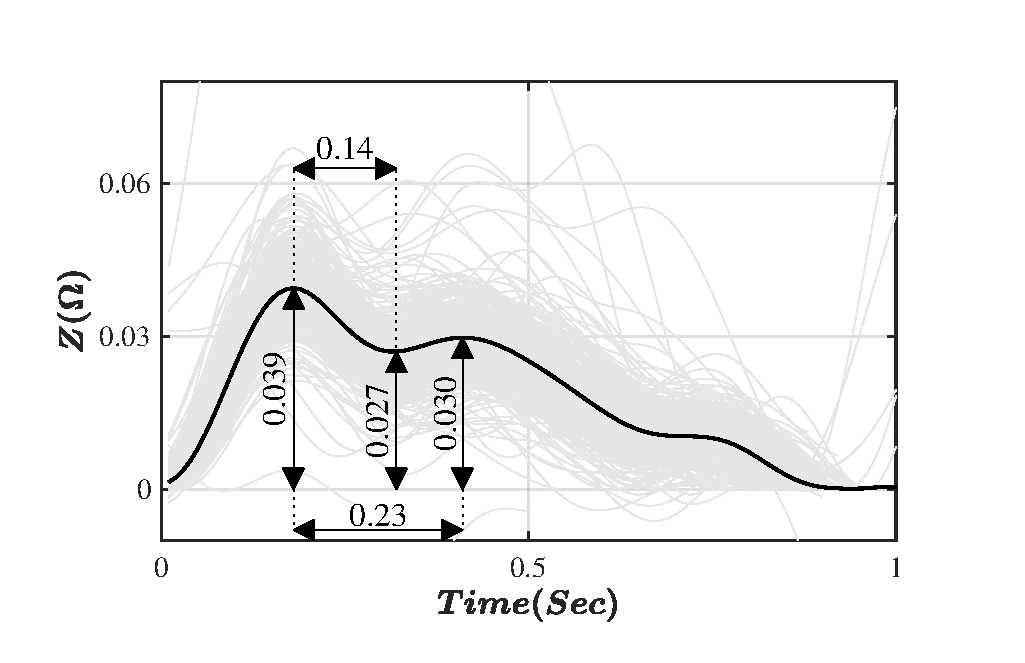
\includegraphics[width=0.45\textwidth, trim={0.5cm 0cm 1.5cm 0 cm}, clip]{figure_apa_4a}}%
	\hfill%
	\subcaptionbox{Average plethysmography waveform during venous occlusion region 4 (\SIrange{780}{960}{\second})\label{fig:iPG arterial occlusion}}
	[0.45\textwidth]{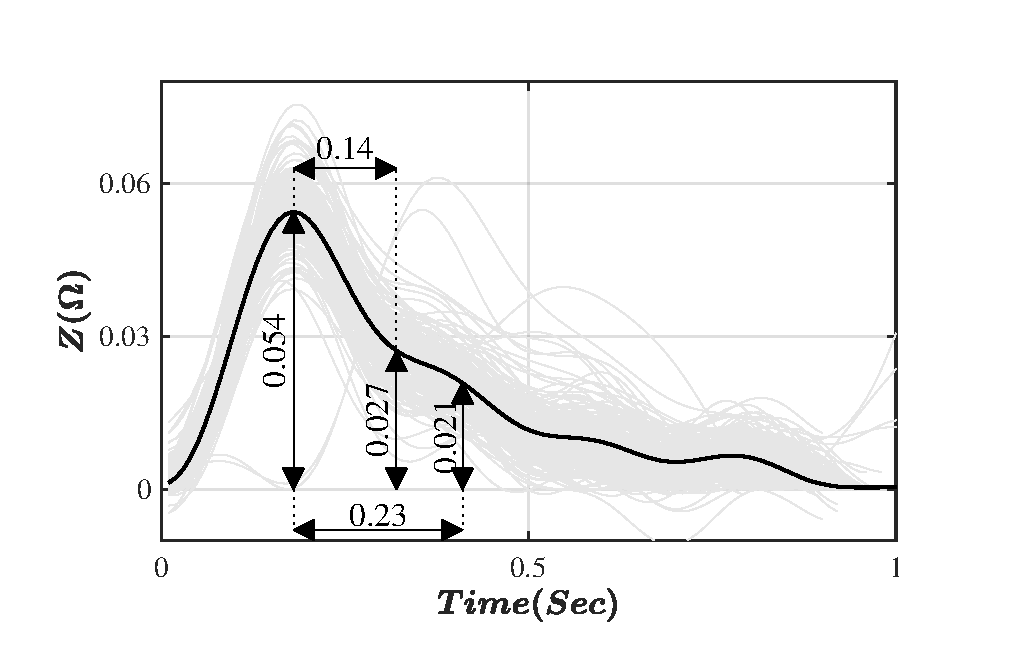
\includegraphics[width=0.45\textwidth, trim={0.5cm 0cm 1.5cm 0 cm}, clip]{figure_apa_4b}}%
	\hfill\null%
	\caption{Plethysmography waveform of the participant seven between baseline and partial arterial occlusion}
	\label{fig:iPG arterial}

	\vspace{1cm}

	\null\hfill%
	\subcaptionbox{Change of amplitude of the waveform at point A.\label{fig:change A arterial}}
	[0.48\textwidth]{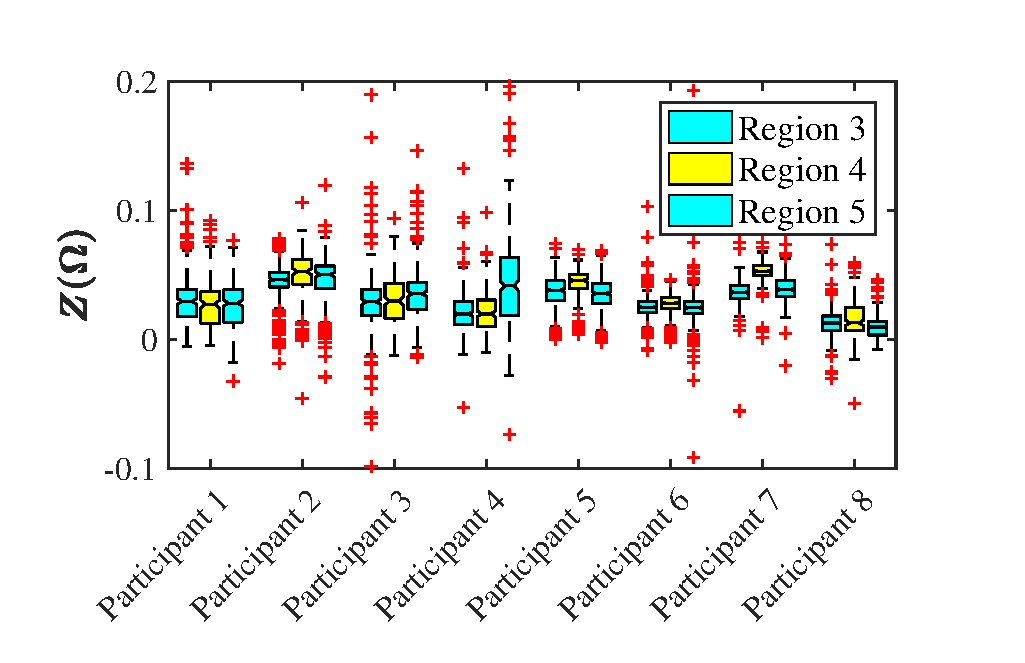
\includegraphics[width=0.45\textwidth, trim={0.5cm 0cm 1.5cm 0 cm}, clip]{figure_apa_5a}}%
	\hfill%
	\subcaptionbox{Change of amplitude of the waveform at point B.\label{fig:change B arterial}}
	[0.48\textwidth]{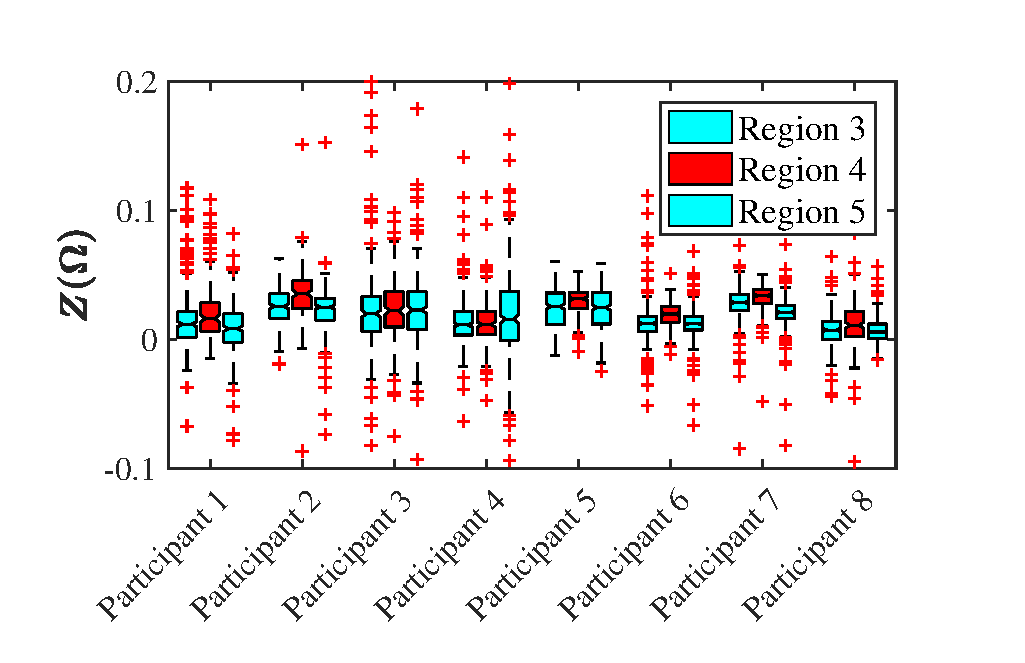
\includegraphics[width=0.45\textwidth, trim={0.5cm 0cm 1.5cm 0 cm}, clip]{figure_apa_5b}}%
	\hfill%
	\subcaptionbox{Change of amplitude of the waveform at point C.\label{fig:change C arterial}}
	[0.48\textwidth]{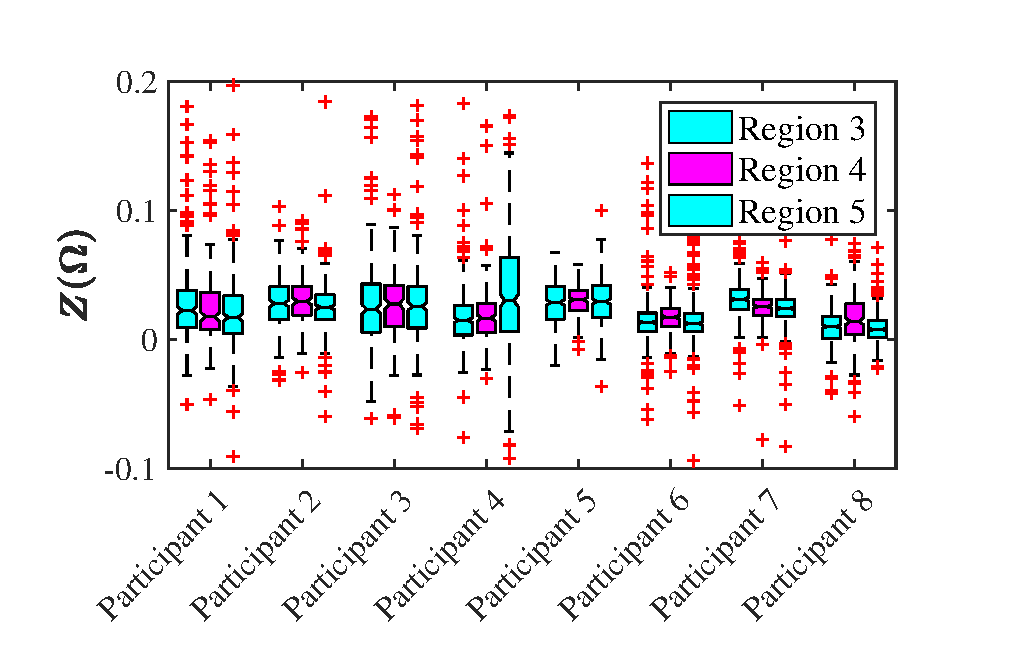
\includegraphics[width=0.45\textwidth, trim={0.5cm 0cm 1.5cm 0 cm}, clip]{figure_apa_5c}}%
	\null%
	\caption{Changes of the impedance peak values during baseline, partial arterial occlusion and return to baseline for points A,B and C.}
	\label{fig:iPG change points arterial}
\end{figure*}

\subsubsection{Changes in systolic peak (Point A)}
\label{section apa 2.2.1}
Figure \ref{fig:change A arterial} indicates the change in amplitude for each one of the participants. Also, table \ref{tbl:change A arterial} summarises the average impedances and the variations in each region. Through this occlusive experiment, 7 participants (\SI{87.5}{\percent}) displayed an increase in electrical resistivity at point A of about \SI{13.52}{\percent}. However, some of these participants showed a tiny increase in their peaks between \SIrange{0.29}{2.24}{\percent}. In general, one can note the hike at this point. After the cuff was deflated, most of the participants (\SI{62.5}{\percent}) showed a decrease of the peak in an average of \SI{-21.86}{\percent}.  In contrast, participants one, three and four registered an increase in their impedance reading, being the later an outlier with an increase in his magnitude of \SI{110.69}{\percent}.

\begin{table}[!htbp]
	\caption{Change of amplitude of the waveform at peak A during the transition from baseline to venous occlusion.}
	\label{tbl:change A arterial}
	\centering\small
	\begin{tabular}{l
					*{3}{S[table-format=1.4]@{\,\( \pm \)\,}S[table-format=1.4]} %Format for Z+-std
					>{\columncolor[gray]{0.8}}c>{\columncolor[gray]{0.9}}c}
		\toprule
		& \multicolumn{2}{c}{\multirow{2}{*}{\textbf{Baseline [\si{\ohm}]}}}
		& \multicolumn{2}{c}{\multirow{2}{*}{\textbf{Occlusion [\si{\ohm}]}}}
		& \multicolumn{2}{c}{\multirow{2}{*}{\textbf{Baseline [\si{\ohm}]}}}
		& \multicolumn{2}{c}{\textbf{Change}} \\
		& \multicolumn{2}{c}{}
		& \multicolumn{2}{c}{}
		& \multicolumn{2}{c}{}
		&\textbf{R3-R4}&\textbf{R4-R5}\\\midrule
	    Participant 1 & 0.0295 & 0.0194 & 0.0274 & 0.0190 & 0.0282 & 0.0265 & -7.03 \% &   2.59 \% \\
		Participant 2 & 0.0462 & 0.0140 & 0.0526 & 0.0197 & 0.0503 & 0.0461 & 13.78 \% &  -5.11 \% \\
		Participant 3 & 0.0292 & 0.0379 & 0.0298 & 0.0185 & 0.0354 & 0.0356 &  2.24 \% &  19.02 \% \\
		Participant 4 & 0.0197 & 0.0242 & 0.0198 & 0.0152 & 0.0416 & 0.0453 &  0.29 \% & 110.69 \% \\
		Participant 5 & 0.0382 & 0.0133 & 0.0458 & 0.0115 & 0.0357 & 0.0351 & 19.81 \% & -26.55 \% \\
		Participant 6 & 0.0249 & 0.0096 & 0.0282 & 0.0081 & 0.0247 & 0.0251 & 13.21 \% & -14.09 \% \\
		Participant 7 & 0.0365 & 0.0097 & 0.0529 & 0.0092 & 0.0388 & 0.0394 & 44.90 \% & -38.73 \% \\
		Participant 8 & 0.0128 & 0.0104 & 0.0128 & 0.0160 & 0.0096 & 0.0098 &  0.38 \% & -24.86 \% \\
		\bottomrule
	\end{tabular}
\end{table}\subsubsection{Changes in dicrotic notch peak (Point B)}
\label{section apa 2.2.2}
In the dicrotic notch position (point B), the increase of its magnitude is clearer than in the systolic peak. In fact, all the participants depicted an increase in their impedance value at this point. Figure \ref{fig:change B arterial} evidence these shifts in each of the regions before and after the occlusion. Table \ref{fig:change B arterial} details participants' median impedances and the ratio of change in each region.

In general, the average increase at the dicrotic notch as soon as the occlusion was applied was about \SI{29.91}{\percent}. When the pressure restricting the blood flow was removed, six out of eight of the study members experienced a fall in electrical resistivity towards baseline. On average, it reduced by \SI{-51.72}{\percent}. Again, participant four was the exception to this reduction, as well as participant three. Their impedance rose by \SI{37.37}{\percent} and \SI{3.25}{\percent} respectively.

\begin{table}[!htbp]
	\caption{Change of amplitude of the waveform at peak B during the transition from baseline to venous occlusion.}
	\label{tbl:change B arterial}
	\centering\small
	\begin{tabular}{l
					*{3}{S[table-format=1.4]@{\,\( \pm \)\,}S[table-format=1.4]} %Format for Z+-std
					>{\columncolor[gray]{0.8}}c>{\columncolor[gray]{0.9}}c}
		\toprule
		& \multicolumn{2}{c}{\multirow{2}{*}{\textbf{Baseline [\si{\ohm}]}}}
		& \multicolumn{2}{c}{\multirow{2}{*}{\textbf{Occlusion [\si{\ohm}]}}}
		& \multicolumn{2}{c}{\multirow{2}{*}{\textbf{Baseline [\si{\ohm}]}}}
		& \multicolumn{2}{c}{\textbf{Change}} \\
		& \multicolumn{2}{c}{}
		& \multicolumn{2}{c}{}
		& \multicolumn{2}{c}{}
		&\textbf{R3-R4}&\textbf{R4-R5}\\\midrule
		Participant 1 & 0.0119 & 0.0232 & 0.0162 & 0.0220 & 0.0083 & 0.0087 & 36.07 \% & -66.02 \% \\
		Participant 2 & 0.0257 & 0.0142 & 0.0354 & 0.0212 & 0.0251 & 0.0231 & 38.02 \% & -40.44 \% \\
		Participant 3 & 0.0200 & 0.0536 & 0.0222 & 0.0247 & 0.0229 & 0.0244 & 11.33 \% &   3.25 \% \\
		Participant 4 & 0.0113 & 0.0256 & 0.0116 & 0.0177 & 0.0158 & 0.0143 &  2.64 \% &  37.37 \% \\
		Participant 5 & 0.0254 & 0.0155 & 0.0314 & 0.0107 & 0.0248 & 0.0237 & 23.55 \% & -26.29 \% \\
		Participant 6 & 0.0124 & 0.0150 & 0.0197 & 0.0096 & 0.0121 & 0.0141 & 58.95 \% & -61.59 \% \\
		Participant 7 & 0.0287 & 0.0128 & 0.0340 & 0.0104 & 0.0211 & 0.0205 & 18.34 \% & -44.99 \% \\
		Participant 8 & 0.0073 & 0.0118 & 0.0110 & 0.0196 & 0.0058 & 0.0069 & 50.41 \% & -71.01 \% \\
\bottomrule
	\end{tabular}
\end{table}

\subsubsection{Changes in diastolic peak (Point C)}
\label{section apa 2.2.3}
Changes in the diastolic peak also presented a similar increasing trend as seen in points A and B. However; the changes were not as marked as the ones seen in the dicrotic notch. Figure \ref{fig:change C arterial} and Table \ref{tbl:change C arterial} summarise the values obtained. In total, \SI{75}{\percent} of the participants showed an increase of impedance between region 3 and 4. It increased with a median of \SI{18.74}{\percent}. Participant eight showed a change significantly larger than the mean (\SI{44.11}{\percent}). Study members one and seven pointed a decrease of electrical resistivity in \SI{-19.91}{\percent} on average.

On the opposite side of the exercise, after releasing the pressure, (\SI{87.5}{\percent}) of the partakers showed a reduction in their impedance, including those whose impedance rose during the occlusion. On average, impedance reduced by \SI{-19.77}{\percent} in total. Again, participant four showed an increase in the ratio of change before and after the blockage significantly exceeding the median of all the measurements. Moreover, this study member outperformed notably the average ratio after the occlusion (\SI{90.32}{\percent}). As portrayed by the other measuring points, this confirms that the data obtained from this study member were not from physiological origin but motion or randomness.

\begin{table}[!htbp]
	\caption{Change of amplitude of the waveform at peak C during the transition from baseline to venous occlusion.}
	\label{tbl:change C arterial}
	\centering\small
	\begin{tabular}{l
					*{3}{S[table-format=1.4]@{\,\( \pm \)\,}S[table-format=1.4]} %Format for Z+-std
					>{\columncolor[gray]{0.8}}c>{\columncolor[gray]{0.9}}c}
		\toprule
		& \multicolumn{2}{c}{\multirow{2}{*}{\textbf{Baseline [\si{\ohm}]}}}
		& \multicolumn{2}{c}{\multirow{2}{*}{\textbf{Occlusion [\si{\ohm}]}}}
		& \multicolumn{2}{c}{\multirow{2}{*}{\textbf{Baseline [\si{\ohm}]}}}
		& \multicolumn{2}{c}{\textbf{Change}} \\
		& \multicolumn{2}{c}{}
		& \multicolumn{2}{c}{}
		& \multicolumn{2}{c}{}
		&\textbf{R3-R4}&\textbf{R4-R5}\\\midrule
	    Participant 1 & 0.0224 & 0.0323 & 0.0176 & 0.0307 & 0.0171 & 0.0206 & -21.35 \% &  -2.21 \% \\
		Participant 2 & 0.0279 & 0.0196 & 0.0295 & 0.0272 & 0.0250 & 0.0252 &   5.96 \% & -16.45 \% \\
		Participant 3 & 0.0236 & 0.0826 & 0.0275 & 0.0284 & 0.0256 & 0.0283 &  16.56 \% &  -7.98 \% \\
		Participant 4 & 0.0149 & 0.0327 & 0.0166 & 0.0229 & 0.0301 & 0.0306 &  11.22 \% &  90.32 \% \\
		Participant 5 & 0.0287 & 0.0171 & 0.0308 & 0.0119 & 0.0293 & 0.0287 &   7.32 \% &  -5.03 \% \\
		Participant 6 & 0.0133 & 0.0252 & 0.0174 & 0.0111 & 0.0123 & 0.0176 &  30.32 \% & -37.72 \% \\
		Participant 7 & 0.0312 & 0.0189 & 0.0254 & 0.0124 & 0.0241 & 0.0232 & -18.48 \% &  -4.27 \% \\
		Participant 8 & 0.0100 & 0.0139 & 0.0141 & 0.0224 & 0.0076 & 0.0087 &  41.11 \% & -64.75 \% \\
		\bottomrule
	\end{tabular}
\end{table}

\subsection{Plethysmography waveform change during total occlusion}
\label{section apa 2.3}
%This method allows multifigures being aligned using subcaptionbox
\begin{figure*}
	\centering
	\null\hfill%
	\subcaptionbox{Average plethysmography waveform during venous occlusion region 5 (\SIrange{960}{1260}{\second})\label{fig:iPG_total_baseline}}
	[0.45\textwidth]{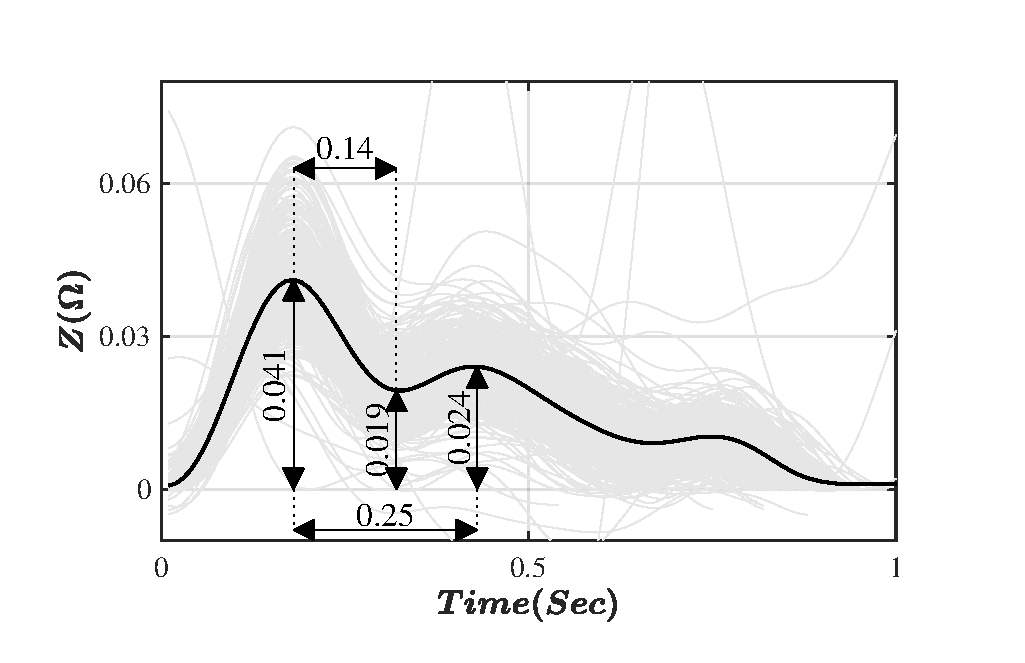
\includegraphics[width=0.45\textwidth, trim={0.5cm 0cm 1.5cm 0 cm}, clip]{figure_apa_6a}}%
	\hfill%
	\subcaptionbox{Average plethysmography waveform during venous occlusion region 6 (\SIrange{1260}{1440}{\second})\label{fig:iPG_total_occlusion}}
	[0.45\textwidth]{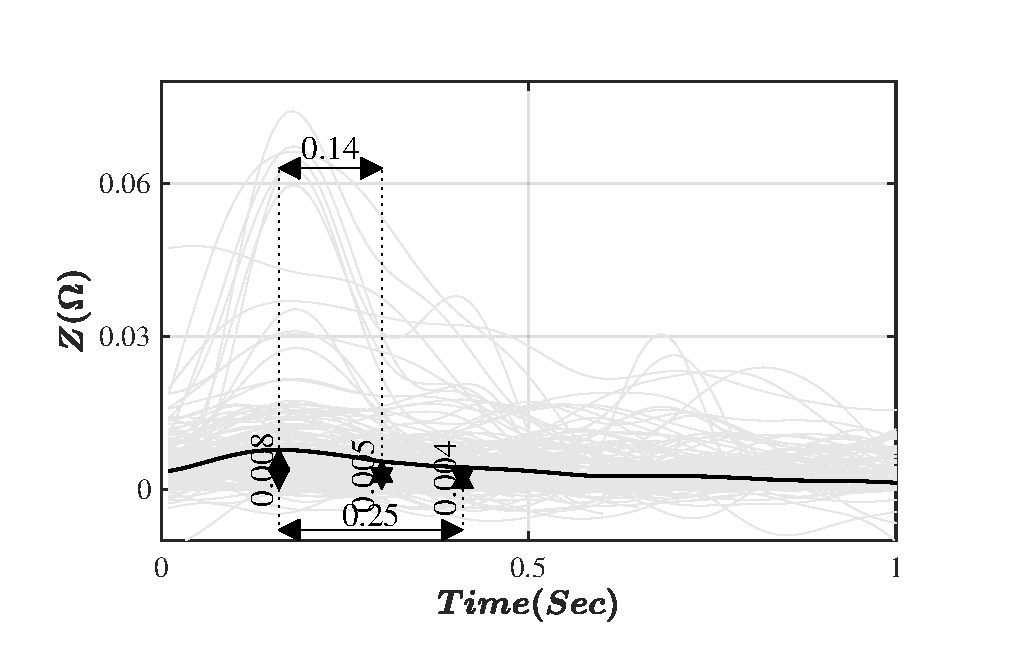
\includegraphics[width=0.45\textwidth, trim={0.5cm 0cm 1.5cm 0 cm}, clip]{figure_apa_6b}}%
	\hfill\null%
	\caption{Plethysmography waveform of the participant seven between baseline and total occlusion}
	\label{fig:iPG_total}
	
	\vspace{1cm}
	
	\null\hfill%
	\subcaptionbox{Change of amplitude of the waveform at point A.\label{fig:change_A_total}}
	[0.48\textwidth]{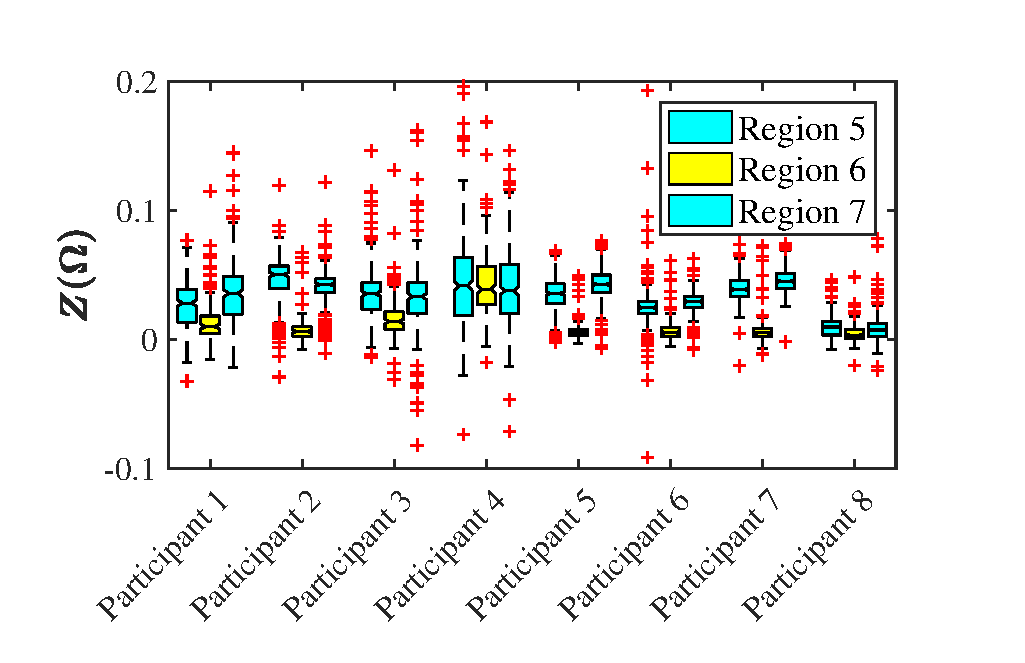
\includegraphics[width=0.45\textwidth, trim={0.5cm 0cm 1.5cm 0 cm}, clip]{figure_apa_7a}}%
	\hfill%
	\subcaptionbox{Change of amplitude of the waveform at point B.\label{fig:change_B_total}}
	[0.48\textwidth]{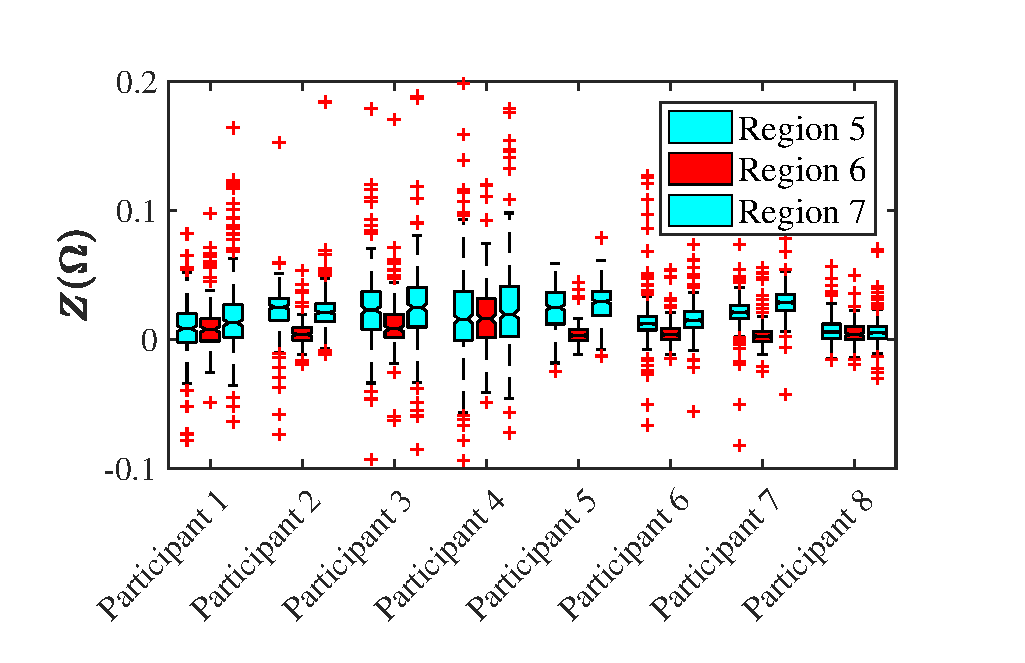
\includegraphics[width=0.45\textwidth, trim={0.5cm 0cm 1.5cm 0 cm}, clip]{figure_apa_7b}}%
	\hfill%
	\subcaptionbox{Change of amplitude of the waveform at point C.\label{fig:change_C_total}}
	[0.48\textwidth]{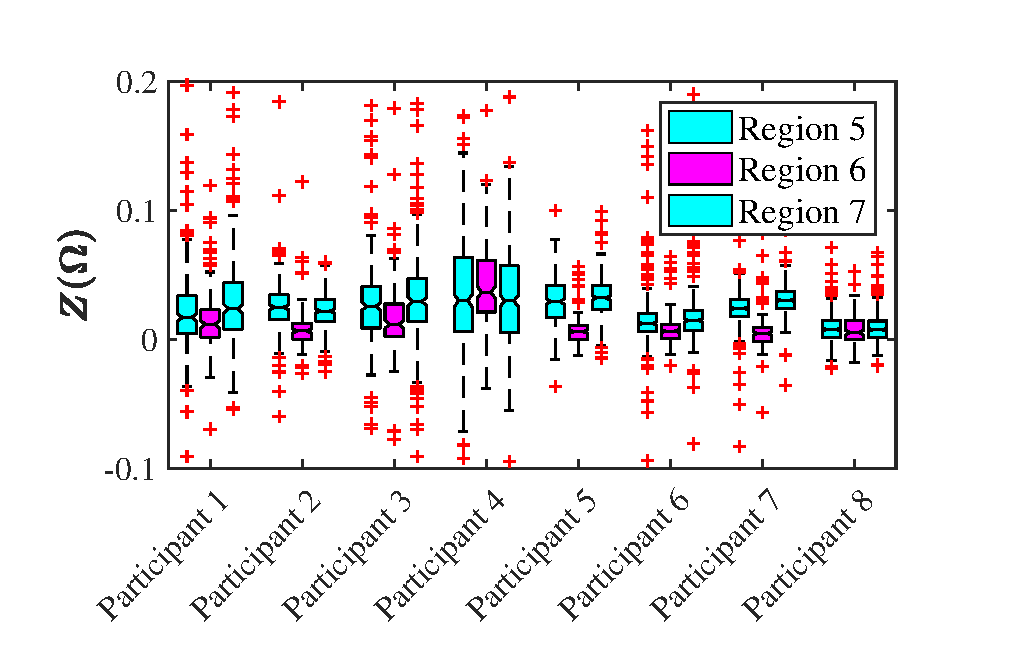
\includegraphics[width=0.45\textwidth, trim={0.5cm 0cm 1.5cm 0 cm}, clip]{figure_apa_7c}}%
	\null%
	\caption{Changes of the impedance peak values during baseline, total occlusion and return to baseline for points A,B and C.}
	\label{fig:iPG_change_points_total}
\end{figure*}

Performing total occlusion completely blocks the inflow and outflow of blood beneath the arm's cuff.  Hence, there is no change of volume within the arm's segment. As a result, impedance plethysmography should not present changes in magnitude.  Figure \ref{fig:iPG_total} shows the APA waveform during baseline in region 5 (\SIrange{960}{1260}{\second}) and all along total occlusion in region 6  (\SIrange{1260}{1440}{\second}) of participant seven. Clearly, as portrayed by figure \ref{fig:iPG_change_points_total}, the amplitudes of most of the participants dropped during the occlusion.However, participant four experienced different behaviour in all these points. The standard deviation of this participant also suggests that there would have been a problem with his plethysmography signal during the test. 

In general, point A decreased on average by \SI{-66.15}{\percent} at its peak value occlusion. Then when the pressure was released, impedance recovered its value in \SI{75.98}{\percent}. A similar event occurred with point B; peak signals dropped a median of \SI{-63.29}{\percent} during blockage and recovered on average by \SI{74.02}{\percent}. Similarly, point C, decreased on average by \SI{-50.27}{\percent}  and increased by \SI{58.71}{\percent} after the occlusion.

%********************************** %Second Section  *************************************
\section{Basal impedance over plethysmography ratio} %Section - 7.2
\label{section discussion 4}

Despite the good level of correlation between DU's amplitude and the iPG's waveform, their blood flow rates do not provide enough details about venous or arterial occlusions. However, the information that the designed iPG device provides seems to present additional details that might give a clue about the kind of circulatory problem. 

As it was described before, the basal impedance has been used to find venous problems by using the venous occlusion technique. However, when an arterial blockage occurs there is a similar response that makes harder to identify where the problem prevails. On the other hand, the amplitude of the impedance plethysmography waveform might provide additional information to discriminate between both kinds of occlusions. Possibly, by combining these two data sets would be possible to discriminate between a right level of circulation and a venous and arterial circulatory problem. 

\begin{figure}[!htpb]
	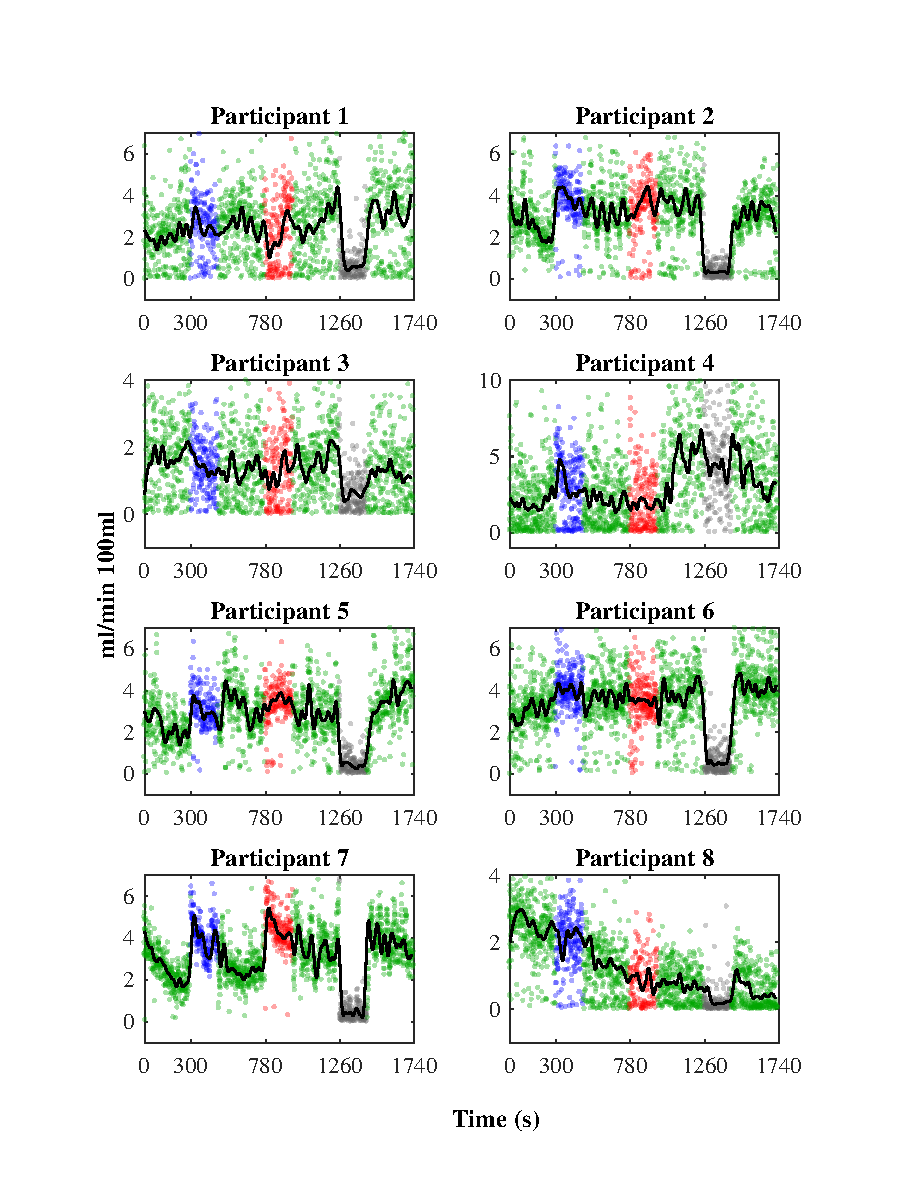
\includegraphics[width=1\textwidth,keepaspectratio]{figure_apa_8}    
	\caption[Ratio of the plethysmography waveform over basal impedance during the experiment]{Measurement of the ratio between the plethysmography waveform over basal impedance during the whole experiment. The blue line represents the systolic peaks, the yellow line the dicrotic notch and the red line the diastolic peak.}
	\label{fig:ratio Z}
\end{figure}

Therefore, it is proposed a ratio indicator between the plethysmography waveform and the basal impedance as a method to differentiate between venous and arterial problems. For this method to work, it is necessary to identify the three points of the plethysmographic waveform, systolic peak, dicrotic notch and diastolic peak. The calculation of the ratio can be performed using the following equation.

\begin{align}
	\label{eq:ratio Z}
	i_Z = \frac{Z_{PG}}{Z_{BAS}}
\end{align}


This is a dimensionless index with three indicators referencing each point of the plethysmography waveform. This method was applied to the participants in the study, and the results were portrayed in figure \ref{fig:ratio Z}. As the graph shows, for most of the data, the systolic peak is over the other two signals. When a venous or partial arterial occlusion occurs (regions 2 and 4), there is an increment in the index. 

The dicrotic notch and the diastolic peak seem to change as a matching pair for most of the baseline signals where the dicrotic notch looks like being slightly lower than the diastolic peak. However, at the time of partial arterial blockage, the systolic index drops below the dicrotic notch index. This event is a clear differentiator between both types of flow restriction.

%********************************** % Third Section  *************************************
\section{Option to evaluate blood obstructions using iPG DC and AC waveforms}  %Section - 7.3 
\label{section discussion 5}
As it was described from the estimation of the blood from the impedance signal could not be a good indicator of circulatory disturbances in either the arterial or venous path. One reason for this, it is that mathematical expression describes there is a direct relation between the amplitude of the wave and the estimation of blood flow. However, when a mechanical constriction of the arm occurs in the venous or arterial circulation the amplitude of the waveform increases. Therefore, this increase in the $\Delta R$ will be calculated as an increase in blood flood which is not altogether correct. 

For this reason, it is proposed a method where it is possible to detect problems in the circulatory path by quantifying and analysing differences in the waveform of the impedance plethysmography signal shape. As it was described in the section \ref{section apa 1}, there are three reference points that can be used to describe an impedance plethysmography waveform. Normally, a non disturbed waveform is represented as systolic peak (point A) higher than the diastolic peak (point C) and the dicrotic notch point (point B) lower than those peaks. 

However, as it has been noticed when a venous occlusion occurs, there are changes in the waveform shape that are distinguishable with each phenomena. The first event that can be noticed is that the systolic peak increases in size. It seems that these gain of size is due to the blood pooling in the veins. Venous occlusion experienced this effect as well as the partial arterial occlusion. However, it must be noticed that partial arterial blockage is also a type of venous occlusion where it restricts the blood flow coming into the forearm. Hence, it is expected to also show an rise in the systolic peak. 

Also, during the venous occlusion can be seen that most of the participants experienced an increase in the magnitude of the dicrotic notch and the diastolic peak. Consequently, it can be said that increase in the impedance plethysmography waveform may represent restriction in the venous circulation towards the forearm. 

Nonetheless, this is not the only indicator of a venous circulatory problem. Likewise, the basal impedance also varies during this kind of occlusion because of the increase of blood volume in the veins. As a result, the basal impedance also decreases in time. Which is also an indicator of circulatory problem. So, presenting these two values in one quantifying number could provide a better indicator of blood flow restriction. 

\begin{figure}[!htpb]
	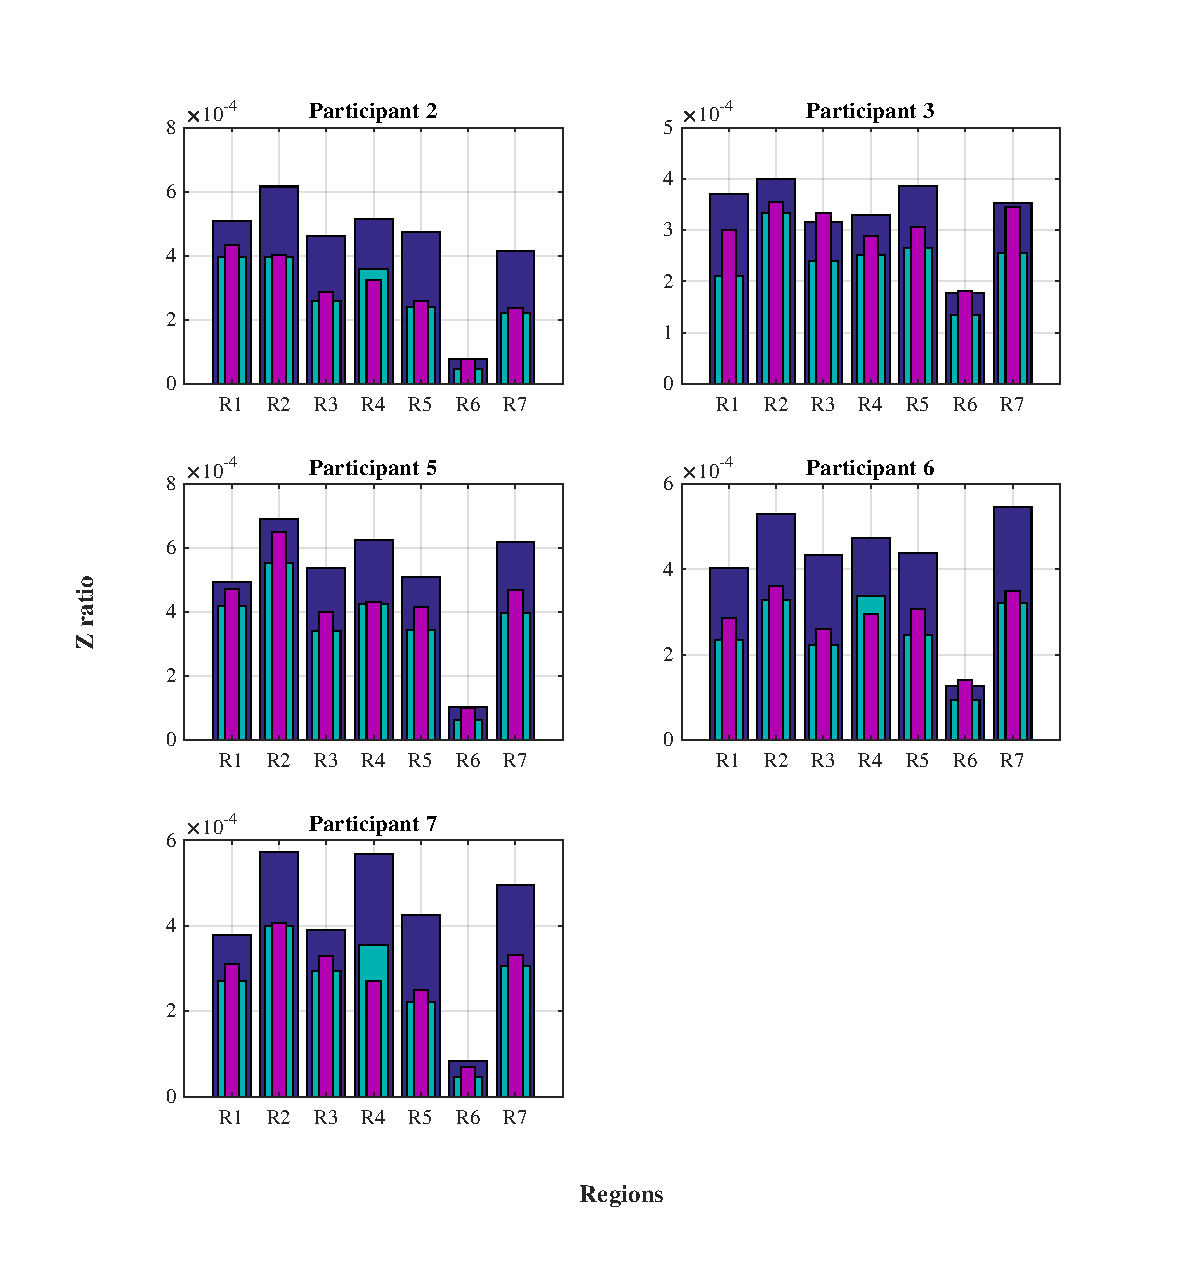
\includegraphics[width=1\textwidth,keepaspectratio]{figure_apa_9}    
	\caption[Bland and Altman plot of the relation between LDF and iPG]{Representation of the index ratio od the APA waveform for each region. The dark purple represents the ratio $\Delta R/ R$ of the systolic peak (point A), the light purple indicates the ratio at the dicrotic notch (point B) and the cyan the magnitude at the diastolic peak (point C).}
	\label{fig:ration Z bar}
\end{figure}

%%********************************** % Section 8.4 ******************************************
\section{Conclusions}
\label{section apa 4}
The iPG signals provided further information about blood distribution during occlusive events. The oscillations of the APA signal comes from the expansion of the arteries and veins during the heart cycle which creates tiny changes in the impedance. This small waveform is contained within the basal impedance but is just a fraction of it. 

The designed impedance device as a whole, including hardware and software algorithms, identified the plethysmography waveforms by localising distinctive landmarks like the systolic peak, dicrotic notch and diastolic point. Obtaining this level of detail was important as provided more features about changes in different parts of the impedance plethysmography waveform. From this premise, it was able to recognise changes in shape during each of the different types of occlusions performed during the test.  Indeed, it is evident that at the time of each occlusive event, the amplitude of the systolic and diastolic peaks manifested a particular response according to the type of blood flow restriction. It must be noted that this waveform shape might be unique to this kind of set-up, changing the electrodes distance or using different frequencies may affect the impedance waveform.

It was observed that there were changes in the size of the systolic peak (point A), dicrotic notch valley (point B) and diastolic peak (point C) when an occlusion occurred. The increase in size might be related to a physiological response during the occlusion where the veins volume capacity increased to receive the pooled blood. An example of this can be seen in figure \ref{fig:iPG change points venous} which showed the differences between region 1, 2 and 3. The figure indicated that there was an increase in the size of all the reference points in most participants during the occlusion followed by a return to baseline. However, the observations from partial occlusion for regions 3,4 and 5 demonstrated that the systolic peak increased in size, but the dicrotic notch and diastolic peak decreased in amplitude compared to venous occlusion and baseline waveform. The difference in the waveform is a clear indicator that an obstruction in either arterial or venous circulation might be occurring. 

The chapter \ref{chapter basal} showed that during the occlusions there is a different slope in each kind of occlusion. By combining the information of the basal impedance and the APA waveform is possible to generate a 3 point ratio index that might indicate a potential obstruction in the forearm. The observation obtained here suggested that if there is a significant increase in the relation index of the systolic peak, it might be the first indicator of circulatory blockage. An increase in the dicrotic notch and the diastolic peak is an indicator that the occlusion might be occurring in the venous return if the dicrotic notch ratio index is higher than the other following one. In comparison, the data collected showed that if systolic peak size increased, but the dicrotic notch amplitude tends to be lower or similar amplitude of the diastolic point, then it might be an indicator that an arterial occlusion might be occurring. 

    



%***** \mynote{Conclusion taken from general conclusion section}
%The iPG signals provide further information about blood distribution during an occlusive events. The oscillations of the APA signal comes from the expansion of the arteries and venous during the heart cycle which creates tiny changes in the impedance. This small signal is contained within the basal impedance but is just a fraction of it. In fact, the contribution of this dynamic signal is just \SI{0.04}{\percent} to the total impedance. Hence, the device described in chapter \ref{chapter design} was able to isolate satisfactory this waveform and provide a high-resolution version of this signal.

%Obtaining this level of detail was important as provided more features about changes in different parts of the impedance plethysmography waveform. The signal collected from this section of the arm gave characteristics of the circulatory process. Three reference points were identified as shown in \ref{section apa 1}. These markers included information about the systolic peak, the dicrotic notch and the diastolic peak which were distinguished by the algorithm implemented. Nonetheless, this waveform is unique to this set-up, changing the electrodes distance or using different frequencies may affect the impedance waveform.

%It was observed that there were changes in the systolic peak (point A), dicrotic notch valley (point B) and diastolic peak (point C) when an occlusion occurs which also affected the blood flow response. During the process described in figure \ref{fig:iPG change points venous} where the changes between region 1, 2 and 3 took place, it can be seen that there is an apparent increase in the size of all the reference points in most participants during the occlusion followed by a return to baseline. 


%%%% General conclusion ideas and outline
%However, this increase of impedance amplitude indicated a raise in the blood flow as reported by chapter \ref{section apa flow arterial pulses} but is not possible to establish whether is an increase in venous or arterial flows. The Doppler ultrasound referenced continuously to the radial artery blood flow. By performing the statistical study shown in \ref{section correlation 2} was established that there is some level of correlation between both signals ($r^2 = 0.35$). Nonetheless, during occlusions, there was a slight difference in the amplitude response. Comparing both flows rate (see figure \ref{fig:DU flow} and figure \ref{fig:blood_flow_plethysmography}) can be noticed that there was more sensitivity from the iPG than the DU at the time of the venous occlusion. From the Doppler ultrasound makes sense that the amplitude of the signal did not show marked changes during this occlusion since the arterial flow was not compromised. Although, the increase in the magnitude of the iPG waveform cannot be related to an increase in arterial flow but might be caused by a venous circulation response to the occlusion and picked up by the impedance device. 

%On the other hand, during the partial arterial occlusion can be seen an alteration in the flow rate recorded by the Doppler ultrasound. The signal's magnitude from this device reduced at the time of this event. When analysing the partial arterial occlusion event (regions 3,4 and 5) described by section \ref{fig:iPG change points arterial} there was also an increase in points A  and B of the signal but point C reduced its amplitude. All these variations were common for most of the participants. The change of the diastolic peak is an indicator of an arterial problem from the waveform obtained. However, at the moment of calculating the blood flow from the impedimetric data a rise in the blood flow was reported which is not utterly concurrent with the DU's measurements. 

%As a conclusion, the iPG device seems capable of measuring blood flow in healthy conditions with a good agreement with the amplitude of Doppler ultrasound measurements. However, there are variations in the basal impedance and the plethysmography waveform shape when a circulatory occlusion is present. In cases where arm's occlusion is not possible the best option is to calculate blood flow changes using the APA waveform. For this reason, monitoring the blood flow solely will not provide enough information to make a clinical decision additional data is required to identify where the real problem lies.


%********************************** %Nomenclature found  *************************************
\nomenclature[z-IPP]{IPP}{Impedance plethysmography pulses}
